

\documentclass[journal]{IEEEtran}

\ifCLASSINFOpdf
\else
\fi

\usepackage{amssymb}
\usepackage{amsthm}
\usepackage{indentfirst}
\usepackage{graphicx}
\usepackage{caption}
\usepackage{algorithm}
\usepackage{algorithmicx}
\usepackage{algpseudocode}
\usepackage{tabularx}
\usepackage{multirow}
\newcommand{\tabincell}[2]{\begin{tabular}{@{}#1@{}}#2\end{tabular}}
\usepackage{array}
\usepackage{booktabs}
\usepackage{multirow}

% correct bad hyphenation here
\hyphenation{op-tical net-works semi-conduc-tor}


\begin{document}

\title{Retinal Vessel Segmentation Using Minimum Spanning Superpixel Tree Detector}

\author{
Zhiwen Qiang, 515030910367 \quad Leqi Zhu, 515020910272 \quad Yulun Wu, 5140719008
}

\maketitle

% As a general rule, do not put math, special symbols or citations
% in the abstract or keywords.
\begin{abstract}
Abstract goes here.
\end{abstract}

% Note that keywords are not normally used for peerreview papers.
\begin{IEEEkeywords}
Keyword 1, keyword 2, keyword 3.
\end{IEEEkeywords}

\IEEEpeerreviewmaketitle

\section{Project Description}

\IEEEPARstart{I}{ntroduction} goes here. 1. The research topics are very popular, very useful, and have great impact and research value

2. The existing methods all have problems, the problems that you are going to solve in the paper

3. Our methods have the theory, therefore our approach can solve the problems in theory as we have the designed

4. Describe the advantages, features, logic, methods, processes, etc. of our methods
 
5. List explicitly 3 to 4 our contributions/advantages like:
Our work makes the following three main contributions:
\begin{itemize}
\item \textbf{Efficient Structure Restoration} The mixed use of different sizes of patches capture the structural information efficiently, avoiding the absorption of irrelevant information which causes abnormal structures;
\item \textbf{Balanced Computational Workload} Multiscale solution with dynamic patches adjusts the computational workload in the operation. It significantly reduces the computation in low pyramid level without sacrificing the visual effects, and accelerates the completing process at the same time;
\item \textbf{Parallel Search \& Competitive Mechanism} Parallel search for different size patches is conducted with GPU acceleration. A competitive mechanism is included to select the patch with minimum unit energy.
\end{itemize}

\section{Pretreatment}
\textbf{Related Work One} XXXXXXXXXX

XXXXXXXXXXXXXXX

XXXXXXXXXXXXXXXXXXXXXXXXX

XXXXXXXXXXXXXXXXXXXXXXXXX

\textbf{Related Work Two} XXXXXXXXXXX

XXXXXXXXXXXXXX

XXXXXXXXXXXXXXXXXXXXXXXXX

XXXXXXXXXXXXXXXXXXXXXXXXX

\textbf{Related Work Three} XXXXXXXXX

XXXXXXXXXXXXXXXX

XXXXXXXXXXXXXXXXXXXXXXXXX


\section{Traditional Methods}
XXXXXXXXXXXXXXXXXXXXXXXXX

Fig. \ref{fig1} shows XXXXX

Fig. \ref{fig5} shows XXXXX

Cite paper like this \cite{Chaudhuri_1989} or like this \cite{Chaudhuri_1989,Li_2014}.

\begin{figure*}
\centering
\footnotesize
\centerline{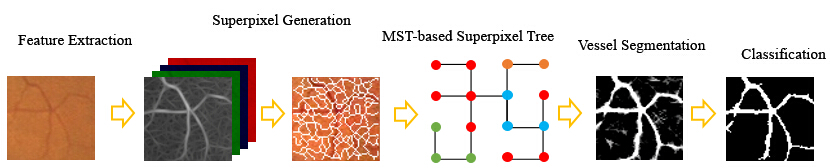
\includegraphics[width=0.9\linewidth]{Fig1.jpg}}
\caption{Overview of the proposed minimum spanning superpixel-based tree detector for retinal vessels.}
\label{fig1}
\end{figure*}

XXXXXXXXXXXXXXXXXXXXXXXXX

\section{Method Part I (at least 7 formulas)}
XXXXXXXXXXXXXXXXXXXXXXXXX

Calculate $a+b=c$ is OK.

\begin{equation} \label{Eq_1}
I(p)= \sum_{q\in\Omega}S(p,q)I(q)=\sum_{q\in\Omega}exp(-\frac{D(p,q)}{\sigma}I(q)
\end{equation}


\renewcommand{\algorithmicrequire}{\textbf{Input:}}
\renewcommand{\algorithmicensure}{\textbf{Output:}}

\begin{algorithm}
	\caption{Dynamic Patch-based Image Completion}
	\label{pseudocode}
	\begin{algorithmic}[1]
		\Require Image $I$ , cavity $C$, source $S=I-C$,
		Number of different size patches $v$,
		Pyramid level $L$
		\Ensure Final Image  $F$
		\State Initialize $F$ through filling patches randomly
		\State Compute image pyramid $I_{l_i}$,$C_{l_i}$,$K(l_i)$, $l_i=L,L-1,\dots,0 $
		
		\For {each pyramid level $l_i$}
		\State Define the patch sizes with Eq. \ref{Eq_1}
		\Repeat
		\For {All $q \in C$}
		\State Parallel Search for $v$ different size patches
		\State Retrieve the patch $P$  that satisfies Eq. \ref{Eq_1}
		\EndFor
		\State Calculate the minimum cost boundary
		\State Combine all the patches
		\Until convergence
		\State Propagate solution to the next level
		
		\EndFor
	\end{algorithmic}\label{holefillalg}
\end{algorithm}


XXXXXXXXXXXXXXXXXXXXXXXXX




\subsection{Test Apple One}
XXXXXXXXXXXXXXXXXXXXXXXXX

XXXXXXXXXXXXXXXXXXXXXXXXX

\subsection{Test Apple Two}
XXXXXXXXXXXXXXXXXXXXXXXXX

XXXXXXXXXXXXXXXXXXXXXXXXX

\subsection{Test Apple Three}
XXXXXXXXXXXXXXXXXXXXXXXXX

XXXXXXXXXXXXXXXXXXXXXXXXX

\section{Method Part II (at least 7 formulas)}
XXXXXXXXXXXXXXXXXXXXXXXXX

XXXXXXXXXXXXXXXXXXXXXXXXX

\subsection{Test Banana One}
XXXXXXXXXXXXXXXXXXXXXXXXX

XXXXXXXXXXXXXXXXXXXXXXXXX

\subsection{Test Banana Two}
XXXXXXXXXXXXXXXXXXXXXXXXX

XXXXXXXXXXXXXXXXXXXXXXXXX

\subsection{Test Banana Three}
XXXXXXXXXXXXXXXXXXXXXXXXX

XXXXXXXXXXXXXXXXXXXXXXXXX

\section{Experimental Results}
XXXXXXXXXXXXXXXXXXXXXXXXX

\begin{figure}
\footnotesize\centering
\centerline{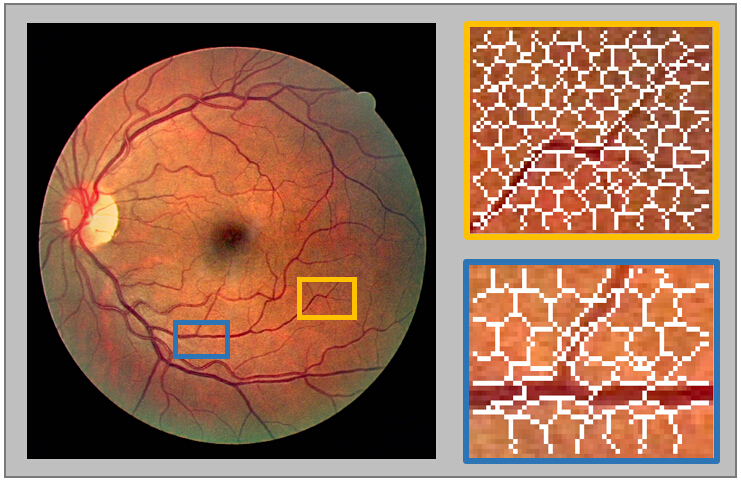
\includegraphics[width=0.8\linewidth]{Fig5.jpg}}\caption{Patches showing the superpixel region after clustering.}
\label{fig5}
\end{figure}


%Cross one column Table
\begin{table}
\centering
\renewcommand\arraystretch{1.2}
\caption{Performance Comparison of Vessel Segmentation}
\begin{tabularx}{0.9\linewidth}{ccccc}
 \toprule
\textbf{Methods} &\textbf{\textit{Connectivity}} &\textbf{\textit{Area}} &\textbf{\textit{Length}} &\textbf{\textit{C*A*L}}
\\ \midrule
2nd Observer &1 &0.9398 &0.9347 &0.8784 \\
Marin \cite{Marin_2011} &0.9990 &0.8327 &0.8314 &0.6916 \\
Soares \cite{Soares} &0.9952 &0.8920 &0.8889 &0.7891 \\
Nguyen \cite{Nguyen_2013} &0.9895 &0.8727 &0.8687 &0.7502 \\
Zhang \cite{Zhang_2010} &0.9988 &0.8097 &0.8108 &0.6557 \\
\textbf{Our method} &\textbf{0.9996} &\textbf{0.9002} &\textbf{0.8982} &\textbf{0.8082} \\
\bottomrule
\end{tabularx}
\end{table}

%Cross two column Table

\begin{table*}[ht]
\caption{Computation time statistics of the evaluations of large CSGs (seconds)}
\label{tab:performance2}
\centering
\begin{tabular}{*{12}{c|}c}%*{4}{>{\centering\arraybackslash}p{35pt}}}
\hline
\multirow{2}{*}{No.} & \multirow{2}{*}{Model} & \multirow{2}{*}{\tabincell{c}{Face \\ Num.}} & \multirow{2}{*}{\tabincell{c}{Mesh \\ Num.}} & \multirow{2}{*}{\tabincell{c}{CGAL}}
& \multirow{2}{*}{\tabincell{c}{Cork}} & \multirow{2}{*}{\tabincell{c}{Carve}} & \multirow{2}{*}{\tabincell{c}{QuickCSG}}&
\multicolumn{5}{c}{Our Approach$^\dag$}\\
 \cline{9-13}
 &&&&&&&& Total & Step 1 & Step 2 & Step 3 & Step 4\\
 \hline\hline
 1 & Organic & 219k & 6 & - & 14.3 & 63.1 & 0.580 & 2.75 & 0.892 & 1.32 & 0.397 & 0.118\\
 2 & T1 & 80k & 50 & 1.00k & 18.5 & 10.4 & 0.388 & 14.4 & 0.691 & 2.71  & 8.11 & 2.87\\
 3 & T2 & 7k & 50 & 2.81k & - & 16.0 & 0.804 & 5.52 & 0.162 & 1.11 & 3.29 & 0.746\\
 4 & Sprocket & 11k & 52 & 211  & - & 4.26 & (0.132)* & 0.386 & 0.093 & 0.105 & 0.149 & 0.034\\
 5 & Ring \& Ball & 146k & 801 & -  & - & 187 & (1.10) & 20.0 & 1.04 & 3.55 & 8.61 & 6.68\\
 \hline
 \end{tabular}
 \end{table*}



XXXXXXXXXXXXXXXXXXXXXXXXX
\section{Deep Learning Methods}
\section{Conclusion and Future Work}
Conclusion goes here.

\ifCLASSOPTIONcaptionsoff
  \newpage
\fi

\bibliographystyle{IEEEtran}
\bibliography{ref}

\end{document}


